\documentclass[10pt]{article}
\usepackage[utf8]{inputenc}

\usepackage{geometry}
\usepackage{graphicx}

\geometry{portrait, margin=1.5in}

\begin{document}
\title{Space Invaders : Sprint 2 Assignment}
\date{\today}
\author{\textit{Group 22}\\ \textit{\underline{TI2206 Software Engineering Methods}} \\
 \\Ege de Bruin \\ Bryan van Wijk \\ Dorian de Koning \\ Jochem Lugtenburg }
 \maketitle  
 \begin{center}
Supervisor: Dr. A. Bacchelli\\
TA: Danny Plenge\\
 \end{center}     
 \begin{center}
 Delft University of Technology\\
 Faculty of EEMCS\\
 \end{center}
 \thispagestyle{empty}
 \pagebreak
 
\section*{Exercise 1 - 20-Time}
\section*{Code improvement requirements}
To improve our code, we want to split several classes into more classes. The classes we want to split are Game and GameUIController, because these classes are now too big in our code. We have chosen to split these classes in the following classes:\\
Game:\newline
\subsection*{Controller}
\begin{itemize}
	\item UnitController
	\item MovingUnitController
	\begin{itemize}
	\item ExplosionController
	\item BarricadeController	
	\item AlienController
	\item SpaceShipController
	\item BulletController
		\begin{itemize}
			\item AlienBulletController
			\item SpaceShipBulletController
		\end{itemize}
	\end{itemize}
\end{itemize}
\subsection*{Unit}
We also want to change the Unit section of our code, we want to have an interface movable that is implemented by the movable/moving. This prevents a lot of duplicate code. Implementing this change would mean we would have to change all of the following classes:
	\begin{itemize}
	\item Unit
	\item Movable
		\begin{itemize}
		\item Alien
		\item SpaceShip
		\item Bullet
		\begin{itemize}
			\item SpaceShipBullet
			\item AlienBullet
		\end{itemize}
		\item Explosion
		\item Barricade
	\end{itemize}
\end{itemize}
\subsection*{GameUiController}
Changing the structure of unit in our code we also need to change the ui section. This will be the new class hierarchy.	
GameUIController:
\begin{itemize}
	\item UiElement
	\begin{itemize}
		\item UiElementUnit
		\begin{itemize}
			\item UiElementAlien
			\item UiElementSpaceShip
			\item UiElementBarricade
			\item UiElementExplosion
			\item UiElementBullet
			\begin{itemize}
				\item UiElementSpaceShipBullet
				\item UiElementAlienBullet
			\end{itemize}
		\end{itemize}
		\item Score
		\item Lives
	\end{itemize}
\end{itemize}
Since we did implement equals methods in most of (the suitable) classes but we did not implement hash code yet. Hashcode should be implemented  too.
\newpage
\section*{Code Improvements classes to be changed}
Each class we split into several subclasses will have one single responsibility. \\
Game:
\subsection*{Controller}
Controller: this interface class will provide template for the Controller classes of different game elements. 
	\begin{itemize}
	\item UnitController: this abstract class has the responsibility of controlling the non moving units in the game
	\item MovingUnitController: this interface has the responsibility of controlling the moving units in the game. 
		\begin{itemize}
			\item ExplosionController: this class is responsible for modifying the explosions in the game.
			\item BarricadeController: this class is responsible for modifying the 	barricades in the game.
			\item AlienController: this class has the responsibility of modifying the aliens in the game.
			\item SpaceShipController: this class is responsible for modifying the spaceship.
			\item BulletController: this class is responsible for modifying the bullets in the game.
			\begin{itemize}
				\item AlienBulletController this class is responsible for modifying the alienbullets in the game.
				\item SpaceShipBulletController this class is responsible for modifying th spaceshipbullets in the game.
			\end{itemize}
		\end{itemize}
	\end{itemize}
\subsection*{Unit}
The change we want to apply to the subclasses of the Unit class is making an interface movable that is implemented by units that move.
\subsection*{GameUiController}
Draw:
\begin{itemize}
	\item UiElement: this (abstract) clas is responsible for drawing all the ui parts on the screen.
	\begin{itemize}
		\item UiElementUnit: this abstract class is responsible for the units on the screen.
			\begin{itemize}
				\item UiElementAlien: this class is responsible for drawing the aliens on the screen.
				\item UiElementSpaceShip: this class is responsible for drawing the spaceship on the screen.
				\item UiElementBarricade: this class is responsible for drawing the barricades on the screen.
				\item UiElementExplosion: this class is responsible for drawing the explosions on the screen.
				\item UiElementBullet: this abstract class is responsible for drawing the bullets on the screen.
				\begin{itemize}
					\item UiElementSpaceShipBullet: this class is responsible for drawing the SpaceShipBullets on the screen.
					\item UiElementShipBullet: this class is responsible for drawing the SpaceShipBullets on the screen.
				\end{itemize}
			\end{itemize}
	\end{itemize}
	\item DrawScore: this class is responsible the score on the screen.
	\item DrawLives: this class is responsible the lives on the screen.
\end{itemize}
\subsection*{Exercise 1 UML} 
\begin{figure}[ht!]
\centering
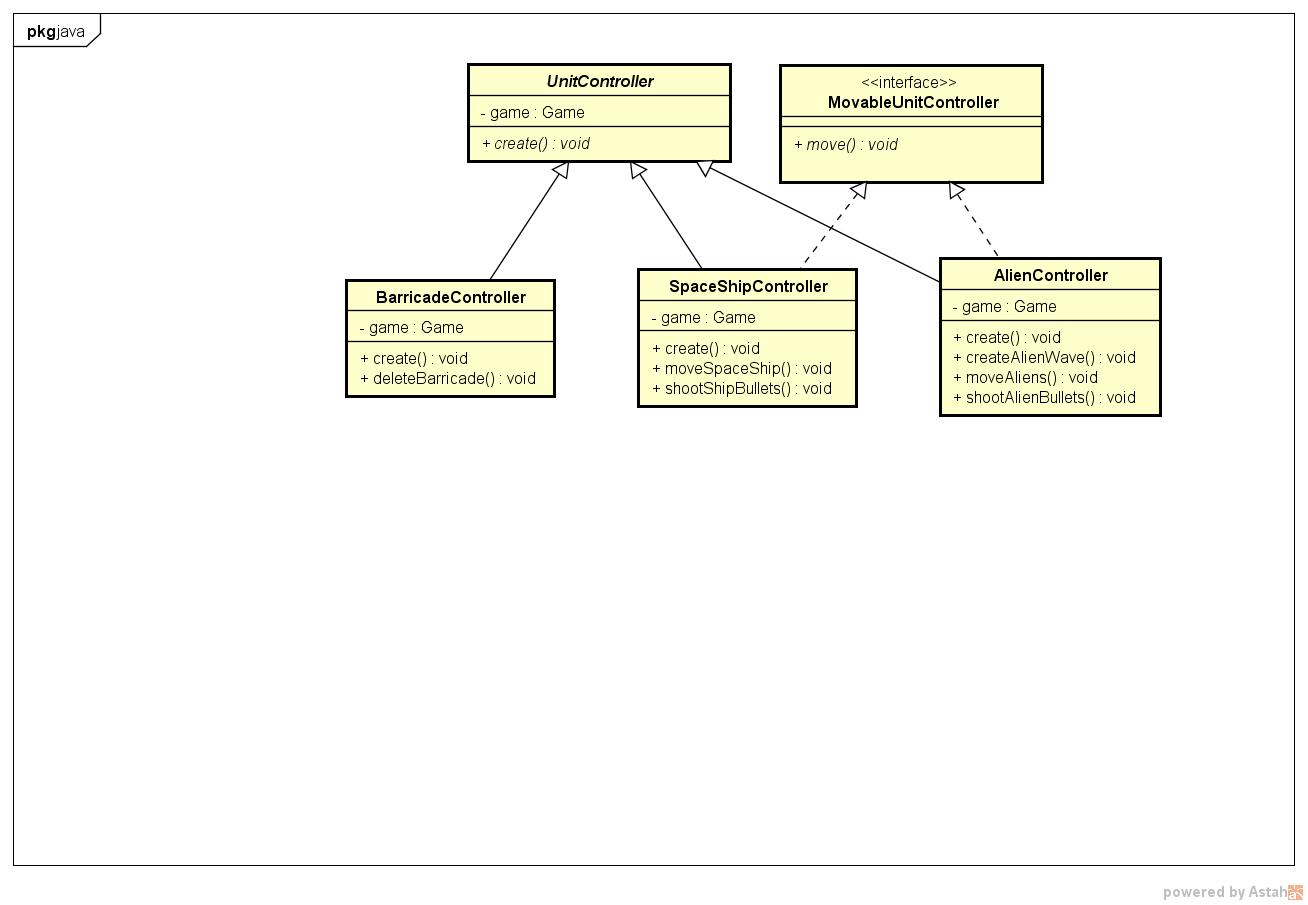
\includegraphics[width=12cm, height=8cm]{ControllerUML.jpg}
\caption{Controller UML Class Diagram}
\end{figure}
\begin{figure}[ht!]
\centering
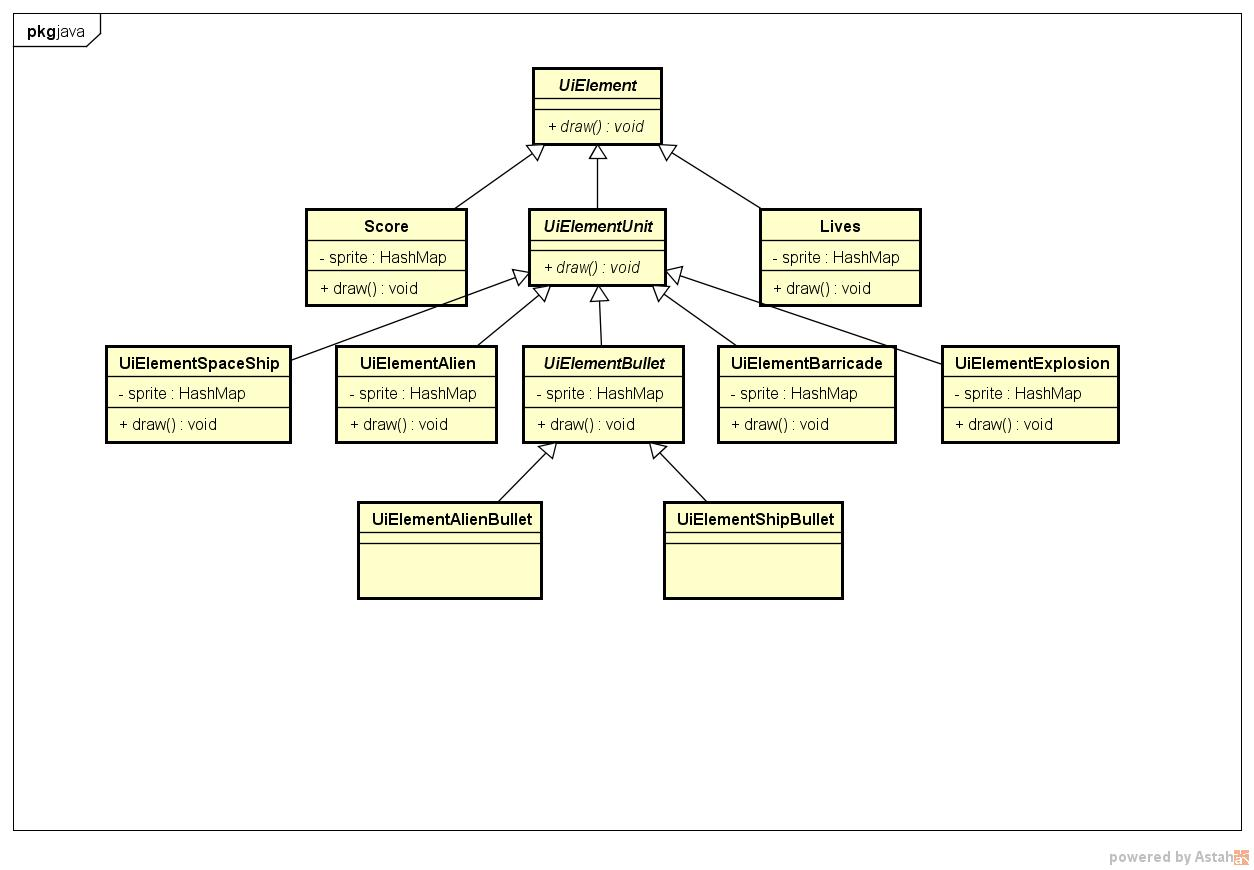
\includegraphics[width=12cm, height=8cm]{UiElementUML.jpg}
\caption{UIElement UML Class Diagram}
\end{figure}
\begin{figure}[ht!]
\centering
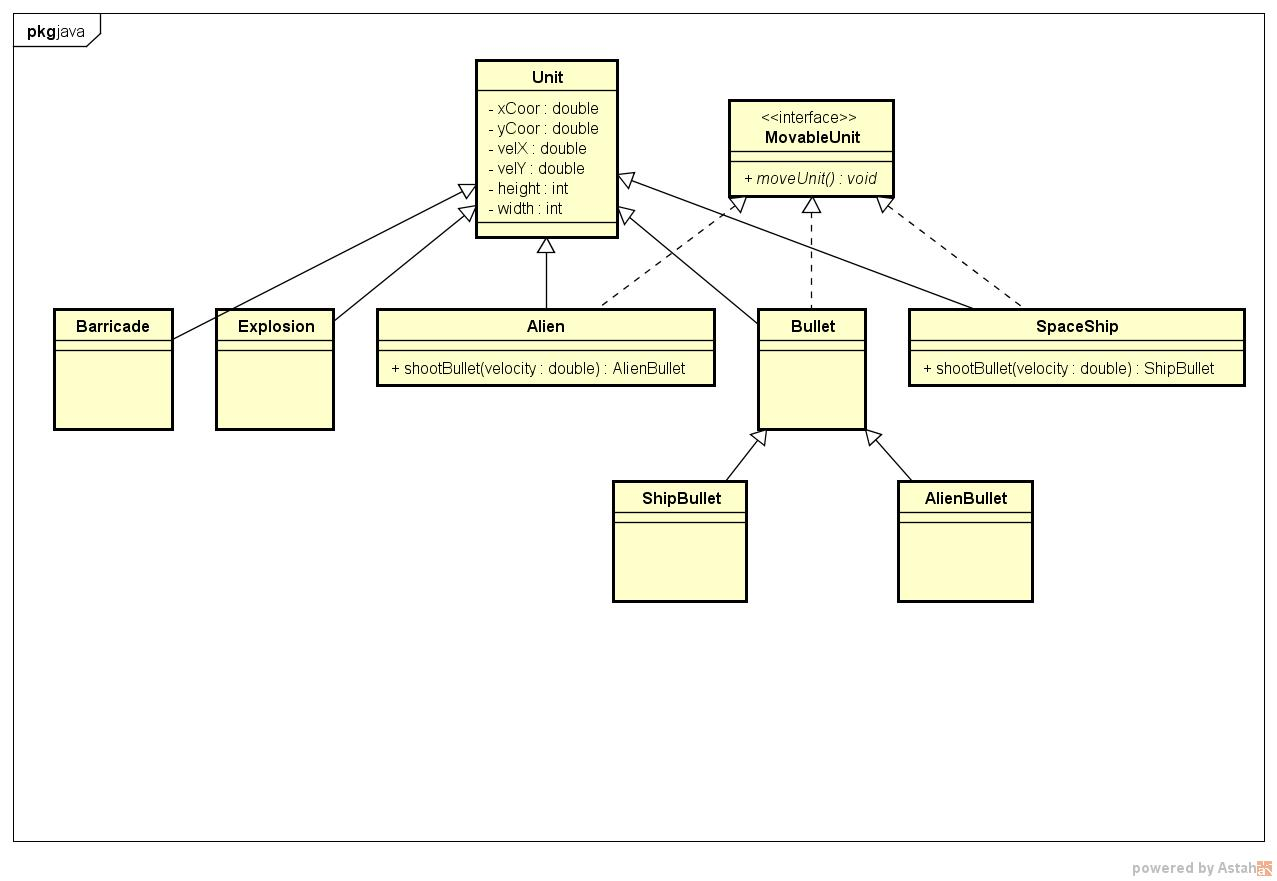
\includegraphics[width=12cm, height=8cm]{UnitUML.jpg}
\caption{Unit UML Class Diagram}
\end{figure}
\pagebreak
\clearpage
\section*{Code Improvement Functional Requirements}

A list of functional requirements considered for code improvements using the MoSCoW method described in the previous section.

\subsection*{Must Haves}
The Code Improvements must meet the following requirements:
\begin{itemize}
	\item Code shall be Checkstyle compliant.
	\item Code shall be PMD and Findbugs compliant.
	\item Classes shall only have one responsibility.
	\item Methods shall not be too long.
\end{itemize}

\subsection*{Should Haves}
The Code Improvements should meet the following requirements:
\begin{itemize}
	\item Code shall contain Javadoc comments explaining complex methods.
	\item Code shall not be commented.
	\item Static shall be used where appropriate.
	\item Private access modifiers shall be used where appropriate.
	\item Test coverage shall be at least 75\%.
	\item Code shall contain less duplicate code.
\end{itemize}

\subsection*{Could Haves}
The Code Improvements could meet the following requirements:
\begin{itemize}
	\item Variables shall be named in correct English.
	\item Methods shall be named in correct English.
	\item Classes shall be named in correct English.
	\item HashCode methods shall be implemented correctly where equals is used.
\end{itemize}

\subsection*{Would/Won't Haves}
The Code Improvements won't meet the following requirements:
\begin{itemize}
	\item ...
\end{itemize}
\newpage
\documentclass[10pt]{article}
\usepackage[utf8]{inputenc}

\usepackage{geometry}
\geometry{portrait, margin=1.5in}

\begin{document}


\section*{Excercise 1}
Each class we split into several subclasses will have one single responsibility. \\
Game:
\begin{itemize}
\item Controller: this interface class will provide template for the Controller classes of different game elements. 
\begin{itemize}
\item UnitController: this abstract class has the responsibility of controlling the non moving units in the game
\begin{itemize}
\item ExplosionController: this class is responsible for modifying the explosions in the game.
\item BarricadeController: this class is responsible for modifying the barricades in the game.
\end{itemize}
\item MovingUnitController: this abstract class is a class that has the responsibility of controlling the moving units in the game. 
\begin{itemize}
	\item AlienController: this class has the responsibility of modifying the aliens in the game.
	\item SpaceShipController: this class is responsible for modifying the spaceship.
	\item BulletController: this class is responsible for modifying the bullets in the game.
	\begin{itemize}
		\item AlienBulletController this class is responsible for modifying the alienbullets in the game.
		\item SpaceShipBulletController this class is responsible for modifying th spaceshipbullets in the game.
	\end{itemize}
\end{itemize}
\end{itemize}
\end{itemize}
GameUIController: \newline
Draw
\begin{itemize}
	\item DrawUnit: this abstract class is responsible for drawing units on the screen.
	\begin{itemize}
		\item DrawAlien: this class is responsible for drawing the aliens on the screen.
		\item DrawSpaceShip: this class is responsible for drawing the spaceship on the screen.
		\item DrawBarricade: this class is responsible for drawing the barricades on the screen.
		\item DrawExplosion: this class is responsible for drawing the explosions on the screen.
		\item DrawBullet: this class is responsible for drawing the bullets on the screen.
	\end{itemize}
	\item DrawScore: this class is responsible the score on the screen.
	\item DrawLives: this class is responsible the lives on the screen.
\end{itemize}
\begin{itemize}
\item Unit: the main class of all units.
\begin{itemize}
\item MovingUnit: the main class of all units that are moving.
\begin{itemize}
\item Alien: this class is the alien unit in the game.
\item SpaceShip: this class is responsible for the spaceship unit.
\item Bullet: this class is responsible for the bullet unit.
\begin{itemize}
\item SpaceShipBullet: this class is responsible for the spaceshipbullet unit.
\item AlienBullet: this class is responsible for the alienbullet unit.
\end{itemize}
\end{itemize}
\item Explosion: this class is responsible for the explosion unit.
\item Barricade: this class is responsible for the barricade unit.
\end{itemize}
\end{itemize}
	
We will use hashcodes to...

\end{document}

\end{document}

